\documentclass[11pt,fleqn, openany]{book} % Default font size and left-justified equations

%%%%%%%%%%%%%%%%%%%%%%%%%%%%%%%%%%%%%%%%%
% The Legrand Orange Book
% Structural Definitions File
% Version 2.1 (26/09/2018)
%
% Original author:
% Mathias Legrand (legrand.mathias@gmail.com) with modifications by:
% Vel (vel@latextemplates.com)
% 
% This file was downloaded from:
% http://www.LaTeXTemplates.com
%
% License:
% CC BY-NC-SA 3.0 (http://creativecommons.org/licenses/by-nc-sa/3.0/)
%
%%%%%%%%%%%%%%%%%%%%%%%%%%%%%%%%%%%%%%%%%

%----------------------------------------------------------------------------------------
%	VARIOUS REQUIRED PACKAGES AND CONFIGURATIONS
%----------------------------------------------------------------------------------------

\usepackage[table]{xcolor}

\usepackage{graphicx}
\usepackage{tabularx} % Required for including pictures
\usepackage{pgf,tikz,tkz-tab,eurosym,yhmath, stmaryrd}
\usepackage{pgfplots}
\usepackage{mathrsfs}
\usetikzlibrary{patterns}
\usetikzlibrary{trees}
\graphicspath{{../../Pictures/}}
\usepackage{multicol} 


\usepackage[english]{babel} % English language/hyphenation
\usepackage{icomma}
\usepackage{enumitem} % Customize lists
\setlist{nolistsep, nosep, nolistsep} % Reduce spacing between bullet points and numbered lists

\usepackage{booktabs} % Required for nicer horizontal rules in tables

 % Required for specifying colors by name


\definecolor{ocre}{RGB}{243,102,25} % Define the orange color used for highlighting throughout the book

\usepackage{listings}

\definecolor{codegreen}{rgb}{0,0.6,0}
\definecolor{codegray}{rgb}{0.5,0.5,0.5}
\definecolor{codepurple}{rgb}{0.58,0,0.82}
\definecolor{backcolour}{rgb}{0.95,0.95,0.92}

\lstdefinestyle{mystyle}{
    backgroundcolor=\color{backcolour},   
    commentstyle=\color{codegreen},
    keywordstyle=\color{magenta},
    numberstyle=\tiny\color{codegray},
    stringstyle=\color{codepurple},
    basicstyle=\ttfamily\footnotesize,
    breakatwhitespace=false,         
    breaklines=true,                 
    captionpos=b,                    
    keepspaces=true,                 
    numbers=left,                    
    numbersep=5pt,                  
    showspaces=false,                
    showstringspaces=false,
    showtabs=false,                  
    tabsize=2
}

\lstset{style=mystyle}

%----------------------------------------------------------------------------------------
% Paramétrage XSIM
%----------------------------------------------------------------------------------------

\usepackage[no-files]{xsim}


\DeclareExerciseEnvironmentTemplate{myex}{%
    \textbf{%
      \hypertarget{ex:\ExerciseID}{\sffamily{\ensuremath{\blacktriangleright}} Exercice \GetExerciseProperty{counter} \GetExerciseProperty{subtitle} --}
      \hyperlink{sol:\ExerciseID}{Voir le corrigé}%
    }\par
}{\par\smallskip}

\DeclareExerciseEnvironmentTemplate{mysol}{%
    \textbf{%
      \hypertarget{sol:\ExerciseID}{\sffamily{\ensuremath{\blacktriangleright}} Correction \GetExerciseProperty{counter} --}
      \hyperlink{ex:\ExerciseID}{Voir l'énoncé}%
    }\par
}{\par\medskip}

\xsimsetup{
  exercise/template = myex ,
  solution/template = mysol 
}

%Collection exercices

\DeclareExerciseTagging{topic}

\xsimsetup{collect}

%----------------------------------------------------------------------------------------
% SYMBOLES
%----------------------------------------------------------------------------------------

\newcommand\imCMsym[4][\mathord]{%
  \DeclareFontFamily{U} {#2}{}
  \DeclareFontShape{U}{#2}{m}{n}{
    <-6> #25
    <6-7> #26
    <7-8> #27
    <8-9> #28
    <9-10> #29
    <10-12> #210
    <12-> #212}{}
  \DeclareSymbolFont{CM#2} {U} {#2}{m}{n}
  \DeclareMathSymbol{#4}{#1}{CM#2}{#3}
}
\newcommand\alsoimCMsym[4][\mathord]{\DeclareMathSymbol{#4}{#1}{CM#2}{#3}}

\imCMsym{cmmi}{124}{\CMjmath}

\newcommand{\Oij}{(O\,;\,\vec{\imath}\,,\, \vec{\CMjmath} )}
\newcommand{\Oijk}{(O\,;\,\vec{\imath}\,,\, \vec{\CMjmath}\,,\,\vec{k})}

\newcommand\e{\mathrm{e}}
\newcommand\R{\mathbb{R}}
\newcommand\N{\mathbb{N}}


%----------------------------------------------------------------------------------------
%	MARGINS
%----------------------------------------------------------------------------------------

\usepackage{geometry} % Required for adjusting page dimensions and margins

\geometry{
	paper=a4paper, % Paper size, change to letterpaper for US letter size
	top=3cm, % Top margin
	bottom=3cm, % Bottom margin
	left=2cm, % Left margin
	right=2cm, % Right margin
	headheight=14pt, % Header height
	footskip=1.4cm, % Space from the bottom margin to the baseline of the footer
	headsep=10pt, % Space from the top margin to the baseline of the header
	%showframe, % Uncomment to show how the type block is set on the page
}

\setlength{\parindent}{0pt}
\parskip=5pt



%----------------------------------------------------------------------------------------
%	FONTS
%----------------------------------------------------------------------------------------

\usepackage{avant} % Use the Avantgarde font for headings
\usepackage{times} % Use the Times font for headings
\usepackage{mathptmx} % Use the Adobe Times Roman as the default text font together with math symbols from the Sym­bol, Chancery and Com­puter Modern fonts

%\usepackage{microtype} % Slightly tweak font spacing for aesthetics
%\usepackage[utf8]{inputenc} % Required for including letters with accents
\usepackage[T1]{fontenc} % Use 8-bit encoding that has 256 glyphs

%----------------------------------------------------------------------------------------
%	BIBLIOGRAPHY AND INDEX
%----------------------------------------------------------------------------------------

\usepackage[style=numeric,citestyle=numeric,sorting=nyt,sortcites=true,autopunct=true,babel=hyphen,hyperref=true,abbreviate=false,backref=true,backend=biber]{biblatex}
\addbibresource{bibliography.bib} % BibTeX bibliography file
\defbibheading{bibempty}{}

\usepackage{calc} % For simpler calculation - used for spacing the index letter headings correctly
\usepackage{makeidx} % Required to make an index
\makeindex % Tells LaTeX to create the files required for indexing

%----------------------------------------------------------------------------------------
%	MAIN TABLE OF CONTENTS
%----------------------------------------------------------------------------------------

\usepackage{titletoc} % Required for manipulating the table of contents

\contentsmargin{0cm} % Removes the default margin

% Part text styling (this is mostly taken care of in the PART HEADINGS section of this file)
\titlecontents{part}
	[0cm] % Left indentation
	{\addvspace{20pt}\bfseries} % Spacing and font options for parts
	{}
	{}
	{}

% Chapter text styling
\titlecontents{chapter}
	[1.25cm] % Left indentation
	{\addvspace{12pt}\large\sffamily\bfseries} % Spacing and font options for chapters
	{\color{ocre!60}\contentslabel[\Large\thecontentslabel]{1.25cm}\color{ocre}} % Formatting of numbered sections of this type
	{\color{ocre}} % Formatting of numberless sections of this type
	{\color{ocre!60}\normalsize\;\titlerule*[.5pc]{.}\;\thecontentspage} % Formatting of the filler to the right of the heading and the page number

% Section text styling
\titlecontents{section}
	[1.25cm] % Left indentation
	{\addvspace{3pt}\sffamily\bfseries} % Spacing and font options for sections
	{\contentslabel[\thecontentslabel]{1.25cm}} % Formatting of numbered sections of this type
	{} % Formatting of numberless sections of this type
	{\hfill\color{black}\thecontentspage} % Formatting of the filler to the right of the heading and the page number

% Subsection text styling
\titlecontents{subsection}
	[1.25cm] % Left indentation
	{\addvspace{1pt}\sffamily\small} % Spacing and font options for subsections
	{\contentslabel[\thecontentslabel]{1.25cm}} % Formatting of numbered sections of this type
	{} % Formatting of numberless sections of this type
	{\ \titlerule*[.5pc]{.}\;\thecontentspage} % Formatting of the filler to the right of the heading and the page number

% Figure text styling
\titlecontents{figure}
	[1.25cm] % Left indentation
	{\addvspace{1pt}\sffamily\small} % Spacing and font options for figures
	{\thecontentslabel\hspace*{1em}} % Formatting of numbered sections of this type
	{} % Formatting of numberless sections of this type
	{\ \titlerule*[.5pc]{.}\;\thecontentspage} % Formatting of the filler to the right of the heading and the page number

% Table text styling
\titlecontents{table}
	[1.25cm] % Left indentation
	{\addvspace{1pt}\sffamily\small} % Spacing and font options for tables
	{\thecontentslabel\hspace*{1em}} % Formatting of numbered sections of this type
	{} % Formatting of numberless sections of this type
	{\ \titlerule*[.5pc]{.}\;\thecontentspage} % Formatting of the filler to the right of the heading and the page number

%----------------------------------------------------------------------------------------
%	MINI TABLE OF CONTENTS IN PART HEADS
%----------------------------------------------------------------------------------------

% Chapter text styling
\titlecontents{lchapter}
	[0em] % Left indentation
	{\addvspace{15pt}\large\sffamily\bfseries} % Spacing and font options for chapters
	{\color{ocre}\contentslabel[\Large\thecontentslabel]{1.25cm}\color{ocre}} % Chapter number
	{}  
	{\color{ocre}\normalsize\sffamily\bfseries\;\titlerule*[.5pc]{.}\;\thecontentspage} % Page number

% Section text styling
\titlecontents{lsection}
	[0em] % Left indentation
	{\sffamily\small} % Spacing and font options for sections
	{\contentslabel[\thecontentslabel]{1.25cm}} % Section number
	{}
	{}

% Subsection text styling (note these aren't shown by default, display them by searchings this file for tocdepth and reading the commented text)
\titlecontents{lsubsection}
	[.5em] % Left indentation
	{\sffamily\footnotesize} % Spacing and font options for subsections
	{\contentslabel[\thecontentslabel]{1.25cm}}
	{}
	{}

%----------------------------------------------------------------------------------------
%	HEADERS AND FOOTERS
%----------------------------------------------------------------------------------------


\usepackage{fancyhdr} % Required for header and footer configuration

\pagestyle{fancy}
\renewcommand{\chaptermark}[1]{\markboth{\sffamily\normalsize\bfseries\ \thechapter.\ #1}{}} % Chapter text font settings
\renewcommand{\sectionmark}[1]{\markright{\sffamily\normalsize\thesection\hspace{5pt}#1}{}} % Section text font settings
\fancyhf{} \fancyhead[LE,RO]{\sffamily\normalsize\thepage} % Font setting for the page number in the header
\fancyhead[LO]{\rightmark} % Print the nearest section name on the left side of odd pages
\fancyhead[RE]{\leftmark} % Print the current chapter name on the right side of even pages

\fancyfoot[L]{Jason LAPEYRONNIE}
\fancyfoot[R]{\href{http://mathoutils.fr}{http://mathoutils.fr}} % Uncomment to include a footer

\renewcommand{\headrulewidth}{0.5pt} % Thickness of the rule under the header
\renewcommand{\footrulewidth}{0.5pt} % Thickness of the rule under the header

\fancypagestyle{plain}{% Style for when a plain pagestyle is specified
	\fancyhead{}\renewcommand{\headrulewidth}{0pt}%
}

% Removes the header from odd empty pages at the end of chapters
\makeatletter
\renewcommand{\cleardoublepage}{
\clearpage\ifodd\c@page\else
\hbox{}
\vspace*{\fill}
\thispagestyle{empty}
\newpage
\fi}

%----------------------------------------------------------------------------------------
%	THEOREM STYLES
%----------------------------------------------------------------------------------------

\usepackage{amsmath,amsfonts,amssymb,amsthm} % For math equations, theorems, symbols, etc

\newcommand{\intoo}[2]{\mathopen{]}#1\,;#2\mathclose{[}}
\newcommand{\ud}{\mathop{\mathrm{{}d}}\mathopen{}}
\newcommand{\intff}[2]{\mathopen{[}#1\,;#2\mathclose{]}}
\renewcommand{\qedsymbol}{$\blacksquare$}
\newtheorem{notation}{Notation}[section]

% Boxed/framed environments
\newtheoremstyle{ocrenumbox}% Theorem style name
{0pt}% Space above
{0pt}% Space below
{\normalfont}% Body font
{}% Indent amount
{\small\bf\sffamily\color{ocre}}% Theorem head font
{\;:\;}% Punctuation after theorem head
{0.25em}% Space after theorem head
{\small\sffamily\color{ocre}\thmname{#1}\nobreakspace\thmnumber{\@ifnotempty{#1}{}\@upn{#2}}% Theorem text (e.g. Theorem 2.1)
\thmnote{\nobreakspace\the\thm@notefont\sffamily\bfseries\color{black}---\nobreakspace#3}} % Optional theorem note

\newtheoremstyle{blacknumex}% Theorem style name
{5pt}% Space above
{10pt}% Space below
{\normalfont}% Body font
{} % Indent amount
{\small\bf\sffamily}% Theorem head font
{\;:\;}% Punctuation after theorem head
{0.25em}% Space after theorem head
{\small\sffamily{\tiny\ensuremath{\blacksquare}}\nobreakspace\thmname{#1}\nobreakspace\thmnumber{\@ifnotempty{#1}{}\@upn{#2}}% Theorem text (e.g. Theorem 2.1)
\thmnote{\nobreakspace\the\thm@notefont\sffamily\bfseries---\nobreakspace#3}}% Optional theorem note

\newtheoremstyle{blacknumexo}% Theorem style name
{15pt}% Space above
{10pt}% Space below
{\normalfont}% Body font
{} % Indent amount
{\small\bf\sffamily}% Theorem head font
{}% Punctuation after theorem head
{0.5em}% Space after theorem head
{\small\sffamily{\ensuremath{\blacktriangleright}}\nobreakspace\thmname{#1}\nobreakspace\thmnumber{\@ifnotempty{#1}{}\@upn{#2}}% Theorem text (e.g. Theorem 2.1)
\thmnote{\nobreakspace\the\thm@notefont\sffamily\bfseries---\nobreakspace#3} \\}% Optional theorem note



\newtheoremstyle{blacknumbox} % Theorem style name
{0pt}% Space above
{5pt}% Space below
{}% Body font
{}% Indent amount
{\large\bf\sffamily}% Theorem head font
{\;:\;}% Punctuation after theorem head
{0.25em}% Space after theorem head
{\small\sffamily\thmname{#1}\nobreakspace\thmnumber{\@ifnotempty{#1}{}\@upn{#2}}% Theorem text (e.g. Theorem 2.1)
\thmnote{\nobreakspace\the\thm@notefont\sffamily\bfseries---\nobreakspace#3}}% Optional theorem note

% Non-boxed/non-framed environments
\newtheoremstyle{ocrenum}% Theorem style name
{5pt}% Space above
{5pt}% Space below
{\normalfont}% Body font
{}% Indent amount
{\small\bf\sffamily\color{ocre}}% Theorem head font
{\;:\;}% Punctuation after theorem head
{0.25em}% Space after theorem head
{\small\sffamily\color{ocre}\thmname{#1}\nobreakspace\thmnumber{\@ifnotempty{#1}{}\@upn{#2}}% Theorem text (e.g. Theorem 2.1)
\thmnote{\nobreakspace\the\thm@notefont\sffamily\bfseries\color{black}---\nobreakspace#3}} % Optional theorem note
\makeatother

% Defines the theorem text style for each type of theorem to one of the three styles above
\newcounter{dummy} 
\newcounter{thm}
\newcounter{correction}
\newcounter{qst}
\theoremstyle{ocrenumbox}
\newtheorem{theoremeT}[dummy]{Théorème}
\newtheorem{exerciseT}{Propriété}
\newtheorem{principeT}{Principe}
\theoremstyle{blacknumex}
\newtheorem{exampleT}{Exemple}
\theoremstyle{blacknumexo}
\newtheorem{exo}[thm]{Exercice}
\newtheorem{corr}[correction]{Correction}
\newtheorem{quest}[qst]{Question}
\theoremstyle{blacknumbox}
\newtheorem{vocabulary}{Vocabulary}[section]
\newtheorem{definitionT}{Définition}
\newtheorem{corollaryT}[dummy]{Corollary}
\theoremstyle{ocrenum}
\newtheorem{proofT}[dummy]{Démonstration}


%----------------------------------------------------------------------------------------
%	DEFINITION OF COLORED BOXES
%----------------------------------------------------------------------------------------

\RequirePackage[framemethod=default]{mdframed} % Required for creating the theorem, definition, exercise and corollary boxes

% Theorem box
\newmdenv[skipabove=7pt,
skipbelow=7pt,
backgroundcolor=black!5,
linecolor=ocre,
innerleftmargin=5pt,
innerrightmargin=5pt,
innertopmargin=10pt,
leftmargin=0cm,
rightmargin=0cm,
innerbottommargin=5pt]{tBox}

%Proposition box	  
\newmdenv[skipabove=7pt,
skipbelow=7pt,
rightline=false,
leftline=true,
topline=false,
bottomline=false,
backgroundcolor=ocre!10,
linecolor=ocre,
innerleftmargin=5pt,
innerrightmargin=5pt,
innertopmargin=10pt,
innerbottommargin=3pt,
leftmargin=0cm,
rightmargin=0cm,
linewidth=4pt]{eBox}	

% Definition box
\newmdenv[skipabove=7pt,
backgroundcolor=ocre!4,
skipbelow=7pt,
rightline=false,
leftline=true,
topline=false,
bottomline=false,
linecolor=ocre,
innerleftmargin=5pt,
innerrightmargin=5pt,
innertopmargin=10pt,
leftmargin=0cm,
rightmargin=0cm,
linewidth=4pt,
innerbottommargin=5pt]{dBox}	

% Corollary box
\newmdenv[skipabove=7pt,
skipbelow=7pt,
rightline=false,
leftline=true,
topline=false,
bottomline=false,
linecolor=gray,
backgroundcolor=black!5,
innerleftmargin=5pt,
innerrightmargin=5pt,
innertopmargin=5pt,
leftmargin=0cm,
rightmargin=0cm,
linewidth=4pt,
innerbottommargin=5pt]{cBox}

\newmdenv[skipabove=7pt,
skipbelow=7pt,
backgroundcolor=black!5,
innerleftmargin=5pt,
topline=false,
bottomline=false,
rightline=false,
leftline=false,
innerrightmargin=5pt,
innertopmargin=5pt,
leftmargin=0cm,
rightmargin=0cm,
innerbottommargin=5pt]{xBox}

% Creates an environment for each type of theorem and assigns it a theorem text style from the "Theorem Styles" section above and a colored box from above
\newenvironment{theorem}{\begin{tBox}\begin{theoremeT}}{\end{theoremeT}\end{tBox}}

\newenvironment{exo2}{\noindent \begin{exo}\item\relax \noindent \begin{eBox}\item\relax}{\end{eBox}\end{exo}}


\newenvironment{proposition}{\begin{eBox}\begin{exerciseT}}{\hfill{\color{ocre}}\end{exerciseT}\end{eBox}}		

\newenvironment{principe}{\begin{eBox}\begin{principeT}}{\hfill{\color{ocre}}\end{principeT}\end{eBox}}	
		  
\newenvironment{definition}{\begin{dBox}\begin{definitionT}}{\end{definitionT}\end{dBox}}	

\newenvironment{example}{\begin{xBox}\begin{exampleT}}{\hfill{\tiny\ensuremath{\blacksquare}}\end{exampleT}\end{xBox}}

\newenvironment{demonstration}{\begin{proofT}}{\hfill{\tiny\ensuremath{\square}}\end{proofT}}		
\newenvironment{corollary}{\begin{cBox}\begin{corollaryT}}{\end{corollaryT}\end{cBox}}	

%----------------------------------------------------------------------------------------
%	REMARK ENVIRONMENT
%----------------------------------------------------------------------------------------

\newenvironment{remark}{\par\vspace{5pt}\small % Vertical white space above the remark and smaller font size
\begin{list}{}{
\leftmargin=25pt % Indentation on the left
\rightmargin=15pt}\item\ignorespaces % Indentation on the right
\makebox[-2.5pt]{\begin{tikzpicture}[overlay]
\node[draw=ocre!60,line width=1pt,circle,fill=ocre!25,font=\sffamily\bfseries,inner sep=2pt,outer sep=0pt] at (-15pt,0pt){\textcolor{ocre}{R}};\end{tikzpicture}} % Orange R in a circle
\advance\baselineskip -1pt}{\end{list}\vskip5pt} % Tighter line spacing and white space after remark

%----------------------------------------------------------------------------------------
%	SECTION NUMBERING IN THE MARGIN
%----------------------------------------------------------------------------------------

\makeatletter
\renewcommand{\@seccntformat}[1]{\llap{\textcolor{ocre}{\csname the#1\endcsname}\hspace{1em}}}                    
\renewcommand{\section}{\@startsection{section}{1}{\z@}
{-4ex \@plus -1ex \@minus -.4ex}
{1ex \@plus.2ex }
{\normalfont\LARGE\sffamily\bfseries}}
\renewcommand{\subsection}{\@startsection {subsection}{2}{\z@}
{-3ex \@plus -0.1ex \@minus -.4ex}
{0.5ex \@plus.2ex }
{\normalfont\sffamily\bfseries}}
\renewcommand{\subsubsection}{\@startsection {subsubsection}{3}{\z@}
{-2ex \@plus -0.1ex \@minus -.2ex}
{.2ex \@plus.2ex }
{\normalfont\small\sffamily\bfseries}}                        
\renewcommand\paragraph{\@startsection{paragraph}{4}{\z@}
{-2ex \@plus-.2ex \@minus .2ex}
{.1ex}
{\normalfont\small\sffamily\bfseries}}

%----------------------------------------------------------------------------------------
%	PART HEADINGS
%----------------------------------------------------------------------------------------

% Numbered part in the table of contents
\newcommand{\@mypartnumtocformat}[2]{%
	\setlength\fboxsep{0pt}%
	\noindent\colorbox{ocre!20}{\strut\parbox[c][.7cm]{\ecart}{\color{ocre!70}\Large\sffamily\bfseries\centering#1}}\hskip\esp\colorbox{ocre!40}{\strut\parbox[c][.7cm]{\linewidth-\ecart-\esp}{\Large\sffamily\centering#2}}%
}

% Unnumbered part in the table of contents
\newcommand{\@myparttocformat}[1]{%
	\setlength\fboxsep{0pt}%
	\noindent\colorbox{ocre!40}{\strut\parbox[c][.7cm]{\linewidth}{\Large\sffamily\centering#1}}%
}

\newlength\esp
\setlength\esp{4pt}
\newlength\ecart
\setlength\ecart{1.2cm-\esp}
\newcommand{\thepartimage}{}%
\newcommand{\partimage}[1]{\renewcommand{\thepartimage}{#1}}%
\def\@part[#1]#2{%
\ifnum \c@secnumdepth >-2\relax%
\refstepcounter{part}%
\addcontentsline{toc}{part}{\texorpdfstring{\protect\@mypartnumtocformat{\thepart}{#1}}{\partname~\thepart\ ---\ #1}}
\else%
\addcontentsline{toc}{part}{\texorpdfstring{\protect\@myparttocformat{#1}}{#1}}%
\fi%
\startcontents%
\markboth{}{}%
{\thispagestyle{empty}%
\begin{tikzpicture}[remember picture,overlay]%
\node at (current page.north west){\begin{tikzpicture}[remember picture,overlay]%	
\fill[ocre!20](0cm,0cm) rectangle (\paperwidth,-\paperheight);
\node[anchor=north] at (4cm,-3.25cm){\color{ocre!40}\fontsize{220}{100}\sffamily\bfseries\thepart}; 
\node[anchor=south east] at (\paperwidth-1cm,-\paperheight+1cm){\parbox[t][][t]{8.5cm}{
\printcontents{l}{0}{\setcounter{tocdepth}{1}}% The depth to which the Part mini table of contents displays headings; 0 for chapters only, 1 for chapters and sections and 2 for chapters, sections and subsections
}};
\node[anchor=north east] at (\paperwidth-1.5cm,-3.25cm){\parbox[t][][t]{15cm}{\strut\raggedleft\color{white}\fontsize{30}{30}\sffamily\bfseries#2}};
\end{tikzpicture}};
\end{tikzpicture}}%
\@endpart}
\def\@spart#1{%
\startcontents%
\phantomsection
{\thispagestyle{empty}%
\begin{tikzpicture}[remember picture,overlay]%
\node at (current page.north west){\begin{tikzpicture}[remember picture,overlay]%	
\fill[ocre!20](0cm,0cm) rectangle (\paperwidth,-\paperheight);
\node[anchor=north east] at (\paperwidth-1.5cm,-3.25cm){\parbox[t][][t]{15cm}{\strut\raggedleft\color{white}\fontsize{30}{30}\sffamily\bfseries#1}};
\end{tikzpicture}};
\end{tikzpicture}}
\addcontentsline{toc}{part}{\texorpdfstring{%
\setlength\fboxsep{0pt}%
\noindent\protect\colorbox{ocre!40}{\strut\protect\parbox[c][.7cm]{\linewidth}{\Large\sffamily\protect\centering #1\quad\mbox{}}}}{#1}}%
\@endpart}
\def\@endpart{\vfil\newpage
\if@twoside
\if@openright
\null
\thispagestyle{empty}%
\newpage
\fi
\fi
\if@tempswa
\twocolumn
\fi}

%----------------------------------------------------------------------------------------
%	CHAPTER HEADINGS
%----------------------------------------------------------------------------------------

% A switch to conditionally include a picture, implemented by Christian Hupfer
\newif\ifusechapterimage
\usechapterimagetrue
\newcommand{\thechapterimage}{}%
\newcommand{\chapterimage}[1]{\ifusechapterimage\renewcommand{\thechapterimage}{#1}\fi}%
\newcommand{\autodot}{.}
\def\@makechapterhead#1{%
{\parindent \z@ \raggedright \normalfont
\ifnum \c@secnumdepth >\m@ne
\if@mainmatter
\begin{tikzpicture}[remember picture,overlay]
\node at (current page.north west)
{\begin{tikzpicture}[remember picture,overlay]
\node[anchor=north west,inner sep=0pt] at (0,0) {\ifusechapterimage\includegraphics[width=\paperwidth]{\thechapterimage}\fi};
\draw[anchor=west] (\Gm@lmargin,-3cm) node [line width=2pt,rounded corners=15pt,draw=ocre,fill=white,fill opacity=0.5,inner sep=15pt]{\strut\makebox[22cm]{}};
\draw[anchor=west] (\Gm@lmargin+.3cm,-3cm) node {\huge\sffamily\bfseries\color{black}\thechapter\autodot~#1\strut};
\end{tikzpicture}};
\end{tikzpicture}
\else
\begin{tikzpicture}[remember picture,overlay]
\node at (current page.north west)
{\begin{tikzpicture}[remember picture,overlay]
\node[anchor=north west,inner sep=0pt] at (0,0) {\ifusechapterimage\includegraphics[width=\paperwidth]{\thechapterimage}\fi};
\draw[anchor=west] (\Gm@lmargin,-3cm) node [line width=2pt,rounded corners=15pt,draw=ocre,fill=white,fill opacity=0.5,inner sep=15pt]{\strut\makebox[22cm]{}};
\draw[anchor=west] (\Gm@lmargin+.3cm,-3cm) node {\huge\sffamily\bfseries\color{black}#1\strut};
\end{tikzpicture}};
\end{tikzpicture}
\fi\fi\par\vspace*{50\p@}}}

%-------------------------------------------

\def\@makeschapterhead#1{%
\begin{tikzpicture}[remember picture,overlay]
\node at (current page.north west)
{\begin{tikzpicture}[remember picture,overlay]
\node[anchor=north west,inner sep=0pt] at (0,0) {\ifusechapterimage\includegraphics[width=\paperwidth]{\thechapterimage}\fi};
\draw[anchor=west] (\Gm@lmargin,-3cm) node [line width=2pt,rounded corners=15pt,draw=ocre,fill=white,fill opacity=0.5,inner sep=15pt]{\strut\makebox[22cm]{}};
\draw[anchor=west] (\Gm@lmargin+.3cm,-3cm) node {\huge\sffamily\bfseries\color{black}#1\strut};
\end{tikzpicture}};
\end{tikzpicture}
\par\vspace*{50\p@}}
\makeatother

%----------------------------------------------------------------------------------------
%	LINKS
%----------------------------------------------------------------------------------------

\usepackage{hyperref}
\hypersetup{hidelinks,backref=true,pagebackref=true,hyperindex=true,colorlinks=false,breaklinks=true,urlcolor=ocre,bookmarks=true,bookmarksopen=false}

\usepackage{bookmark}
\bookmarksetup{
open,
numbered,
addtohook={%
\ifnum\bookmarkget{level}=0 % chapter
\bookmarksetup{bold}%
\fi
\ifnum\bookmarkget{level}=-1 % part
\bookmarksetup{color=ocre,bold}%
\fi
}
}

\renewcommand*\thesection{\arabic{section}}

\newcommand*{\coord}[3]{% 
  \ensuremath{\overrightarrow{#1}\, 
    \begin{pmatrix} 
      #2\\ 
      #3 
    \end{pmatrix}}}
    
  \newcommand*{\coordb}[2]{% 
  \ensuremath{ 
    \begin{pmatrix} 
      #1\\ 
      #2 
    \end{pmatrix}}}

\newcommand*{\coorde}[4]{% 
  \renewcommand{\arraystretch}{1}\ensuremath{\overrightarrow{#1}\, 
    \begin{pmatrix} 
      #2\\ 
      #3 \\
      #4
    \end{pmatrix}}}    
  \newcommand*{\coordbe}[3]{% 
 \renewcommand{\arraystretch}{1} \ensuremath{ 
    \begin{pmatrix} 
      #1\\ 
      #2 \\
      #3
    \end{pmatrix}}}  
    
\newcommand{\Card}{\mathrm{Card}}


\begin{document}

\chapterimage{../../Pictures/background}

\chapter{Cours : Rappels de probabilité}



Avant de s'engager sur le programme de terminale, faisons quelques rappels de probabilités de l'année de Première.

Dans tout ce chapitre, on note $\Omega$ l'univers non vide d'une expérience aléatoire.\\
On rappelle que pour deux événements $A$ et $B$ de $\Omega$, l'événement $A \cap B$ est l'événement qui est réalisé lorsque « à la fois $A$ et $B$ sont réalisés ».\\De plus, l'événement $\bar{A}$, appelé contraire de $A$, est réalisé si et seulement si $A$ ne l'est pas.

$\mathbb{P}(A)$ désignera la probabilité de l'événement $A$. On a alors $\mathbb{P}(\overline{A})=1-\mathbb{P}(A)$.


\section{Probabilité conditionnelle}

\begin{definition}[Probabilité conditionnelle]Soit $A$ et $B$ deux événements tels que $\mathbb{P}(A)\neq 0$. On appelle probabilité conditionnelle de $B$ sachant $A$, la quantité
\[ \mathbb{P}_A(B)=\dfrac{\mathbb{P}(A\cap B)}{\mathbb{P}(A)}.\]\end{definition}

\begin{example} On considère l'univers $\Omega = \{ 1;2;3;4;5;6\}$. On tire un nombre uniformément au hasard sur $\Omega$. On  considère les événements
\begin{itemize}
\item $A$ : le nombre est pair ;
\item $B$ : le nombre est supérieur ou égal à 3.
\end{itemize}
Puisque l'on est en situation d'équiprobabilité, on a alors $\mathbb{P}(A)=\qquad\qquad$ et $\mathbb{P}(B)=$\\
Par ailleurs, $A\cap B = \qquad $. Ainsi, $\mathbb{P}(A \cap B) = $\\
Appliquant la définition, on trouve donc 
\[ \mathbb{P}_A(B)=\dfrac{\mathbb{P}(A\cap B)}{\mathbb{P}(A)}=\qquad\qquad\qquad
\text{et} 
\quad \mathbb{P}_B(A)=\dfrac{\mathbb{P}(B\cap A)}{\mathbb{P}(B)}=\]
\end{example}

Cette probabilité s'interprète comme la probabilité de l'événement $B$ sachant que l'événement $A$ est réalisé.

\begin{example}Une entreprise commande à une société de sondage une enquête sur la satisfaction de ses clients. Lors du premier appel téléphonique, la probabilité qu'un client réponde est de 0,25. Si le client répond à l'appel, la probabilité qu'il réponde au questionnaire de la société est de 0,3. On note $R$ l'événement « la personne répond à l'appel » et $Q$ l'événement « la personne répond au questionnaire ». 

D'après l'énoncé, on a $\mathbb{P}(R)=\qquad\qquad$ et $\mathbb{P}_R(Q)=\qquad\qquad$. Ainsi, la probabilité qu'une personne prise au hasard réponde à l'appel puis au questionnaire vaut $\mathbb{P}(R \cap Q) = \mathbb{P}(R) \times \mathbb{P}_R(Q)=$\end{example}

\newpage

\subsection{Construction d'un arbre pondéré}

\begin{proposition}[Règle de la somme] Dans un arbre pondéré, la somme des probabilités issues d'un nœud est égale à 1.
\end{proposition}

\begin{example} On considère une succession de deux expériences aléatoires dont l'arbre pondéré associé est représenté ci-dessous.
\tikzstyle{level 1}=[level distance=3.5cm, sibling distance=4cm]
\tikzstyle{level 2}=[level distance=3.5cm, sibling distance=1.5cm]
\tikzstyle{level 3}=[level distance=3.5cm, sibling distance=0.3cm]

% Define styles for bags and leafs
\tikzstyle{bag} = [text width=4em, text centered]
\tikzstyle{end} = [circle, minimum width=3pt,fill, inner sep=0pt]


\begin{center}
\begin{tikzpicture}[scale=0.8,grow=right,sloped]
\node[bag] { }
    child {
        node[bag] {C} 
        child {
                node[bag] {F}
                edge from parent node[below] {$0,3$}
            }
        child {
               node[bag] {E}
               edge from parent node[above] {$0,4$}
            }
        child {
                node[bag] {D}
                edge from parent [very thick, red]
            }
            edge from parent node[above] {$0,6$} 
    }
    child {
        node[bag] {B}        
            child {
                node[bag] {F}
                edge from parent [black] node[below] {$0,2$}
            }
            child {
                node[bag] {E}
                 child{
                	node[bag] {$B\cap E$}
                	edge from parent [dashed,->]
                	}
                edge from parent [black] node[above] {$0,4$}
            }
            child {
                node[bag] {D}
                edge from parent [black] node[above] {$0,4$}
            }
            edge from parent [thick, blue]
    }
     child {
        node[bag] {A}        
            child {
                node[bag] {F}
                edge from parent node[below] {$0,1$}
            }
            child {
                node[bag] {E}
                edge from parent node[above] {$0,1$}
            }
            child {
                node[bag] {D}
                child{
                	node[bag] {$A\cap D$}
                	edge from parent [dashed,->]
                	}
                edge from parent node[above] {$0,8$}
            }
            edge from parent node[above] {$0,3$}
        };
\end{tikzpicture}
\end{center}



\begin{itemize}
\item Sur cet arbre, on voit que $\mathbb{P}(A)=\qquad\qquad$ et $\mathbb{P}(C)=$
\item Puisque la somme des probabilités issues d'une branche vaut 1, on a $\mathbb{P}(A)+\mathbb{P}(B)+\mathbb{P}(C)=1$, soit $\mathbb{P}(B)=$
\item La probabilité conditionnelle $\mathbb{P}_A(D)$ se lit sur la branche qui relie $A$ à $D$. Ainsi, $\mathbb{P}_A(D)=$.
\item La somme des probabilités issues du nœud $C$ doit valoir 1. \\ On a donc $\mathbb{P}_C(D)+\mathbb{P}_C(E)+\mathbb{P}_C(F)=1$. Ainsi, $\mathbb{P}_C(D)=$
\end{itemize}\end{example}


\begin{proposition}[Règle du produit] Dans un arbre pondéré la probabilité d'une issue est égale au produit des probabilités du chemin aboutissant à cette issue
\end{proposition}

\begin{example}Pour obtenir l'issue $A\cap D$, on passe par les sommets $A$ puis $D$.

On a alors $\mathbb{P}(A\cap D)=$\end{example}

On retrouve la relation $\mathbb{P}(A \cap D)= \mathbb{P}(A) \times \mathbb{P}_A(D)$.
\newpage
\subsection{Formule des probabilités totales}

\begin{definition}[Partition]Soit $\Omega$ l'univers d'une expérience aléatoire. \\On dit que les événements $A_1$, $A_2$, ..., $A_n$ forment une partition de $\Omega$ lorsque
\begin{itemize}
\item Les ensembles $A_1$, $A_2$, ..., $A_n$ sont non vides ;
\item Les ensembles $A_1$, $A_2$, ..., $A_n$ sont deux à deux disjoints ;
\item $A_1\cup A_2\cup \ldots \cup A_n = \Omega$.
\end{itemize}
Dans le cadre des probabilités, on parle également de \textbf{système complet d'événements}.\end{definition}

\begin{example}On considère $\Omega = \{1;2;3;4;5;6;7;8\}$ ainsi que les événements $A_1=\{1;3\}$, \\ $A_2=\{2;4;5;6;7\}$ et $A_3=\{8\}$. $A_1$, $A_2$ et $A_3$ forment une partition de $\Omega$.\end{example}

\begin{proposition}[Formule des probabilités totales] On considère un événement $B$ et une partition $A_1$, $A_2$, ..., $A_n$ de l'univers $\Omega$. Alors,
\[ \mathbb{P}(B)=\mathbb{P}(B \cap A_1) + \mathbb{P}(B \cap A_2) + \ldots + \mathbb{P}(B \cap A_n) = \sum_{i=1}^{n} \mathbb{P}(B\cap A_i).\]
\end{proposition}


\begin{example} On reprend l'exemple de la partie précédente. On souhaite calculer la probabilité $\mathbb{P}(D)$. Pour cela, on regarde l'ensemble des branches qui contiennent l'événement $D$.

\tikzstyle{level 1}=[level distance=3.5cm, sibling distance=4cm]
\tikzstyle{level 2}=[level distance=3.5cm, sibling distance=1.5cm]
\tikzstyle{level 3}=[level distance=3.5cm, sibling distance=0.3cm]

% Define styles for bags and leafs
\tikzstyle{bag} = [text width=4em, text centered]
\tikzstyle{end} = [circle, minimum width=3pt,fill, inner sep=0pt]


\begin{center}
\begin{tikzpicture}[scale=0.7,grow=right,sloped]
\node[bag] { }
    child {
        node[bag] {C} 
        child {
                node[bag] {F}
                edge from parent node[below] {$0.3$}
            }
        child {
               node[bag] {E}
               edge from parent node[above] {$0.4$}
            }
        child {
                node[bag] {D}
                child{
                	node[bag] {$C\cap D$}
                	edge from parent [dashed,->]
                	}
                edge from parent node[above] {$0.3$}
            }
            edge from parent node[above] {$0.6$} 
    }
    child {
        node[bag] {B}        
            child {
                node[bag] {F}
                edge from parent [black] node[below] {$0.2$}
            }
            child {
                node[bag] {E}
                edge from parent [black] node[above] {$0.4$}
            }
            child {
                node[bag] {D}
                    child{
                	node[bag] {$B\cap D$}
                	edge from parent [dashed,->]
                	}
                edge from parent [black] node[above] {$0.4$}
            }
            edge from parent node[above] {$0.1$}
    }
     child {
        node[bag] {A}        
            child {
                node[bag] {F}
                edge from parent node[below] {$0.1$}
            }
            child {
                node[bag] {E}
                edge from parent node[above] {$0.1$}
            }
            child {
                node[bag] {D}
                child{
                	node[bag] {$A\cap D$}
                	edge from parent [dashed,->]
                	}
                edge from parent node[above] {$0.8$}
            }
            edge from parent node[above] {$0.3$}
        };
\end{tikzpicture}
\end{center}

\begin{itemize}
\item $A$, $B$ et $C$ forment une partition de $\Omega$.
\item On a $\mathbb{P}(D)=\mathbb{P}(A\cap D) + \mathbb{P}(B\cap D) + \mathbb{P}(C\cap D)$. De plus,
\begin{itemize}
\item $\mathbb{P}(A\cap D)=$ 
\item $\mathbb{P}(B\cap D)=$ 
\item $\mathbb{P}(C\cap D)=$
\end{itemize}
\item Ainsi, $\mathbb{P}(D)=$
\end{itemize}
\vspace{-0.5cm}
\end{example}


\section{Variable aléatoire réelle}

\subsection{Variable aléatoire}

\begin{definition}On appelle variable aléatoire réelle toute fonction définie sur l'univers $\Omega$ d'une expérience aléatoire et à valeurs dans $\mathbb{R}$.\\
Les variables aléatoires sont en général notées $X$.\end{definition}

\begin{minipage}{0.55\linewidth}\begin{example}On choisit un nombre entier au hasard entre 1 et 6 compris. L'univers de l'expérience aléatoire est donc l'ensemble $\{1;2;3;4;5;6\}$.

Si le nombre obtenu est 6, on gagne 2 points. Si le nombre est impair, on perd 1 point. Dans les autres cas, on ne gagne ni ne perd aucun point.\\
On appelle $X$ la variable aléatoire qui donne le nombre de points gagnés selon le résultat.
\begin{itemize}
\item Si on obtient le nombre 1, on perd 1 point. \\On a ainsi $X(1)=$.
\item Si on obtient le nombre 6, on gagne 2 points. \\On a ainsi $X(6)=$.
\item On a également $X(2)=\qquad\qquad$, $X(3)=\qquad\qquad$, $X(4)=\qquad\qquad$ et $X(5)=\qquad\qquad$.
\end{itemize}\end{example}
\end{minipage}\hfill\begin{minipage}{0.43\linewidth}

\tikzstyle{level 1}=[level distance=2.5cm, sibling distance=1.5cm]
\tikzstyle{level 2}=[level distance=4.2cm, sibling distance=1.5cm]
\tikzstyle{level 3}=[level distance=3.5cm, sibling distance=0.3cm]

% Define styles for bags and leafs
\tikzstyle{bag} = [text width=4em, text centered]
\tikzstyle{end} = [circle, minimum width=3pt,fill, inner sep=0pt]


\begin{center}
\begin{tikzpicture}[scale=0.8,grow=right,sloped]
\draw (3,5) node {\textbf{Univers}};
\draw (7,5) node {\textbf{Variable}};
\draw (7,4.8) node[below] {\textbf{aléatoire}};
\node[bag] { }
    child {
        node[bag] {6} 
        child {
                node[bag] {2}
                edge from parent[dashed,->,>=latex] node[below] {$ $}
            }
            edge from parent node[above] {$ $} 
    }
	child {
        node[bag] {5} 
        child {
                node[bag] {$-1$}
                edge from parent[dashed,->,>=latex] node[below] {$ $}
            }
            edge from parent node[above] {$ $} 
    }
    child {
        node[bag] {4} 
        child {
                node[bag] {0}
                edge from parent[dashed,->,>=latex] node[below] {$ $}
            }
            edge from parent node[above] {$ $} 
    }
    child {
        node[bag] {3} 
        child {
                node[bag] {$-1$}
                edge from parent[dashed,->,>=latex] node[below] {$ $}
            }
            edge from parent node[above] {$ $} 
    }
    child {
        node[bag] {2} 
        child {
                node[bag] {0}
                edge from parent[dashed,->,>=latex] node[below] {$ $}
            }
            edge from parent node[above] {$ $} 
    }
    child {
        node[bag] {1} 
        child {
                node[bag] {$-1$}
                edge from parent[dashed,->,>=latex] node[below] {$ $}
            }
            edge from parent node[above] {$ $} 
    }
    ;
\end{tikzpicture}
\end{center}\end{minipage}


\begin{definition}Soit $X$ une variable aléatoire réelle sur un univers $\Omega$ et $a$ un réel.\\
On note $\{X=a\}$ l'événement qui regroupe toutes les issues $\omega$ de $\Omega$ telle que $X(\omega)=a$.\\
On peut définir de la même manière les événements $\{X<a\}$, $\{X\leqslant a\}$, $\{X\geqslant a\}$...\end{definition}

\begin{example}On reprend l'exemple précédent.
\begin{itemize}
\item L'événement $\{X=-1\}$ correspond aux issues qui font perdre un point, soit les issues
\item L'événement $\{X\geqslant 0\}$ correspond aux issues qui font gagner 0 point ou plus, soit les issues
\end{itemize}\end{example}

\subsection{Loi d'une variable aléatoire}


\begin{definition}Soit $X$ une variable aléatoire réelle sur un univers fini $\Omega$.\\
La loi de probabilité de $X$ est la fonction qui, à chaque réel $k$, associe la probabilité  $\mathbb{P}(X=k)$.\end{definition}

On rappelle que \textbf{la somme des probabilités doit valoir 1} !

\begin{example}On choisit uniformément au hasard un nombre entier entre 1 et 8 compris.

\begin{itemize}
\item Si le nombre obtenu est supérieur ou égal à 6, on gagne 2 points.
\item Si le nombre obtenu est inférieur ou égal à 4, on perd 3 points.
\item Si le nombre obtenu est 5, on gagne 5 points.
\end{itemize}
On note $X$ la variable aléatoire qui donne le nombre de points gagnés après l'expérience.\\


\tikzstyle{level 1}=[level distance=3.5cm, sibling distance=1cm]
\tikzstyle{level 2}=[level distance=5cm, sibling distance=1.5cm]
\tikzstyle{level 3}=[level distance=3.5cm, sibling distance=0.3cm]

% Define styles for bags and leafs
\tikzstyle{bag} = [text width=4em, text centered]
\tikzstyle{end} = [circle, minimum width=3pt,fill, inner sep=0pt]


\begin{center}
\begin{tikzpicture}[scale=0.8,grow=right,sloped]
\draw (3.5,4.5) node {\textbf{Univers}};
\draw (8.5,4.5) node {\textbf{Variable aléatoire $X$}};
\node[bag] { }
	child {
        node[bag] {8} 
        child {
                node[bag] {$2$}
                edge from parent[dashed,->,>=latex] node[below] {$ $}
            }
            edge from parent node[above] {$ $} 
    }
    child {
        node[bag] {7} 
        child {
                node[bag] {$2$}
                edge from parent[dashed,->,>=latex] node[below] {$ $}
            }
            edge from parent node[above] {$ $} 
    }
    child {
        node[bag] {6} 
        child {
                node[bag] {2}
                edge from parent[dashed,->,>=latex] node[below] {$ $}
            }
            edge from parent node[above] {$ $} 
    }
	child {
        node[bag] {5} 
        child {
                node[bag] {$5$}
                edge from parent[dashed,->,>=latex] node[below] {$ $}
            }
            edge from parent node[above] {$ $} 
    }
    child {
        node[bag] {4} 
        child {
                node[bag] {$-3$}
                edge from parent[dashed,->,>=latex] node[below] {$ $}
            }
            edge from parent node[above] {$ $} 
    }
    child {
        node[bag] {3} 
        child {
                node[bag] {$-3$}
                edge from parent[dashed,->,>=latex] node[below] {$ $}
            }
            edge from parent node[above] {$ $} 
    }
    child {
        node[bag] {2} 
        child {
                node[bag] {$-3$}
                edge from parent[dashed,->,>=latex] node[below] {$ $}
            }
            edge from parent node[above] {$ $} 
    }
    child {
        node[bag] {1} 
        child {
                node[bag] {$-3$}
                edge from parent[dashed,->,>=latex] node[below] {$ $}
            }
            edge from parent node[above] {$1/8$} 
    }
    ;
\end{tikzpicture}
\end{center}

$X$ peut donc prendre trois valeurs : $-3$, $2$ ou $5$. 

Pour déterminer la loi de $X$, il faut donc déterminer $\mathbb{P}(X=-3)$, $\mathbb{P}(X=2)$ et $\mathbb{P}(X=5)$.
\begin{itemize}
\item L'événement $\{X=-3\}$ est composé des issues 1, 2, 3 et 4. \\ Puisque l'on est en situation d'équiprobabilité, $\mathbb{P}(X=-3)=\dfrac{4}{8}=\dfrac{1}{2}$.
\vskip5pt
\item L'événement $\{X=2\}$ est composé des issues 6, 7 et 8. \\ Puisque l'on est en situation d'équiprobabilité, $\mathbb{P}(X=2)=\dfrac{3}{8}$.
\vskip5pt
\item L'événement $\{X=5\}$ est composé de l'issue 5. \\ Puisque l'on est en situation d'équiprobabilité, $\mathbb{P}(X=-3)=\dfrac{1}{8}$.
\end{itemize}
On peut résumer la loi de la variable aléatoire $X$ dans un tableau.
\renewcommand{\arraystretch}{2.2}
\begin{center}
\begin{tabular}{|l|c|c|c|}
\hline
$k$ & $-3$ & $2$ & $5$ \\
\hline
$\mathbb{P}(X=k)$ & $\dfrac{1}{2}$ & $\dfrac{3}{8}$ & $\dfrac{1}{8}$ \\
\hline \end{tabular}
\end{center}
\end{example}


\subsection{Espérance d'une variable aléatoire réelle}

\begin{definition}Soit $X$ une variable aléatoire. On note $x_1$, $x_2$, ..., $x_n$ les valeurs prises par $X$.\\
Pour $i$ allant de $1$ à $n$, on note $p_i$ la probabilité $\mathbb{P}(X=x_i)$. L'espérance de $X$, notée $E[X]$, est la valeur
\[ E[X]= p_1x_1+p_2x_2+\ldots + p_n x_n = \sum _{i=1}^{n} p_i x_i.\]\end{definition}

Il s'agit en quelque sorte de la moyenne des valeurs prises par la variable aléatoire $X$, pondérées par leurs probabilités. Nous verrons dans un prochain chapitre que le terme de moyenne prendra tout son sens...
\newpage
\begin{example}On considère une variable aléatoire $X$ dont la loi est donnée par le tableau suivant.

\renewcommand{\arraystretch}{2.2}
\begin{center}
\begin{tabular}{|l|c|c|c|c|}
\hline
$k$ & $-1$& $2$ & $3$ & $8$ \\
\hline
$\mathbb{P}(X=k)$ & $\dfrac{1}{3}$ & $\dfrac{1}{4}$ & $\dfrac{1}{6}$ & $\dfrac{1}{4}$\\
\hline \end{tabular}
\end{center}


L'espérance de la variable aléatoire $X$ vaut :
\[ E[X]=\]

« En moyenne », la variable aléatoire $X$ vaut \end{example}

\subsection{Variance et écart-type d'une variable aléatoire réelle}

\begin{definition}Soit $X$ une variable aléatoire. On note $x_1$, $x_2$, ..., $x_n$ les valeurs prises par la variable aléatoire $X$.
La variance $X$, notée $V(X)$, est la valeur
\[ V(X)= p_1(x_1-E[X])^2+p_2(x_2-E[X])^2+\ldots + p_n( x_n-E[X])^2 = \sum _{i=1}^{n} p_i (x_i-E[X])^2.\]
Cette quantité mesure la dispersion de la variable aléatoire autour de l'espérance.\end{definition}

\textbf{Remarque :} On a en fait $V(X)= E[ (X-E[X])^2 ]$.

\begin{example}On considère une variable aléatoire $X$ dont la loi est donnée par le tableau suivant.

\renewcommand{\arraystretch}{2.2}
\begin{center}
\begin{tabular}{|l|c|c|c|c|}
\hline
$k$ & $-3$& $1$ & $4$ & $9$ \\
\hline
$\mathbb{P}(X=k)$ & $0.6$ & $0.2$ & $0.15$ & $0.05$\\
\hline \end{tabular}
\end{center}

Dans un premier temps, on calcule l'espérance de la variable aléatoire $X$.
\[E[X] =\]

Pour calculer la variance,
\begin{itemize}
\item Pour chaque valeur de la variable aléatoire, on retire l'espérance. On dit que l'on centre la variable aléatoire ;
\item On met chaque nombre obtenu au carré ;
\item Chaque nombre est multiplié par sa probabilité ;
\item On ajoute alors chacun des nombres obtenus.
\end{itemize}
\newpage
Dans ce cas,
\renewcommand{\arraystretch}{2.2}
\begin{center}
\begin{tabularx}{0.9 \linewidth}{|l|X|X|X|X|}
\hline
$x_i$ & $-3$& $1$ & $4$ & $9$ \\
\hline
$x_i-E[X]$ & &  &  &  \\
\hline
$(x_i-E[X])^2$ & &  &  & \\
\hline
$p_i$ & $0.6$ & $0.2$ & $0.15$ & $0.05$\\
\hline
$p_i(x_i-E[X])^2$ &  &  &  & \\
\hline \end{tabularx}
\end{center}

La variance de $X$ vaut donc 
\[ V(X) =\]\end{example}

\begin{proposition}[Formule de König-Huygens]
Soit $X$ une variable aléatoire. On a alors
\[V(X)=E[X^2]-(E[X])^2.\]
\end{proposition}

\begin{example}
Reprenons l'exemple précédent. Pour déterminer la loi de $X^2$, il suffit de mettre les valeurs prises par la variable aléatoire au carré. On a alors

\renewcommand{\arraystretch}{2.2}
\begin{center}
\begin{tabularx}{0.9\linewidth}{|l|X|X|X|X|}
\hline
$k$ & &  & & \\
\hline
$\mathbb{P}(X^2=k)$ &  &  &  & \\
\hline \end{tabularx}
\end{center}

Ainsi, $E[X^2]=$

On a donc $V(X)=E[X^2]-(E[X])^2=$ 

On retrouve bien la valeur précédente.

\end{example}

\begin{definition} Soit $X$ une variable aléatoire réelle. On appelle écart-type de $X$, noté $\sigma(X)$ (sigma), la valeur
\[ \sigma (X)= \sqrt{V(X)}.\]\end{definition}

L'écart-type mesure la "variation moyenne" de la variable aléatoire autour de l'espérance.

\begin{example}Dans l'exemple précédent, l'écart-type était donc $\sigma(X)=$\end{example}







\end{document}